\subsection{FHR Benchmark Specifications}

\subsection{FHR Benchmark Results}

\begin{frame}
    \frametitle{FHR Benchmark Phase I-A Results}
    \begin{table}
        \only<1,3-4>{\caption{FHR Benchmark Phase I-A (2D assembly steady state model) results 
        \cite{chee_arfcfhr-benchmark_2021}.}}
        \only<1>{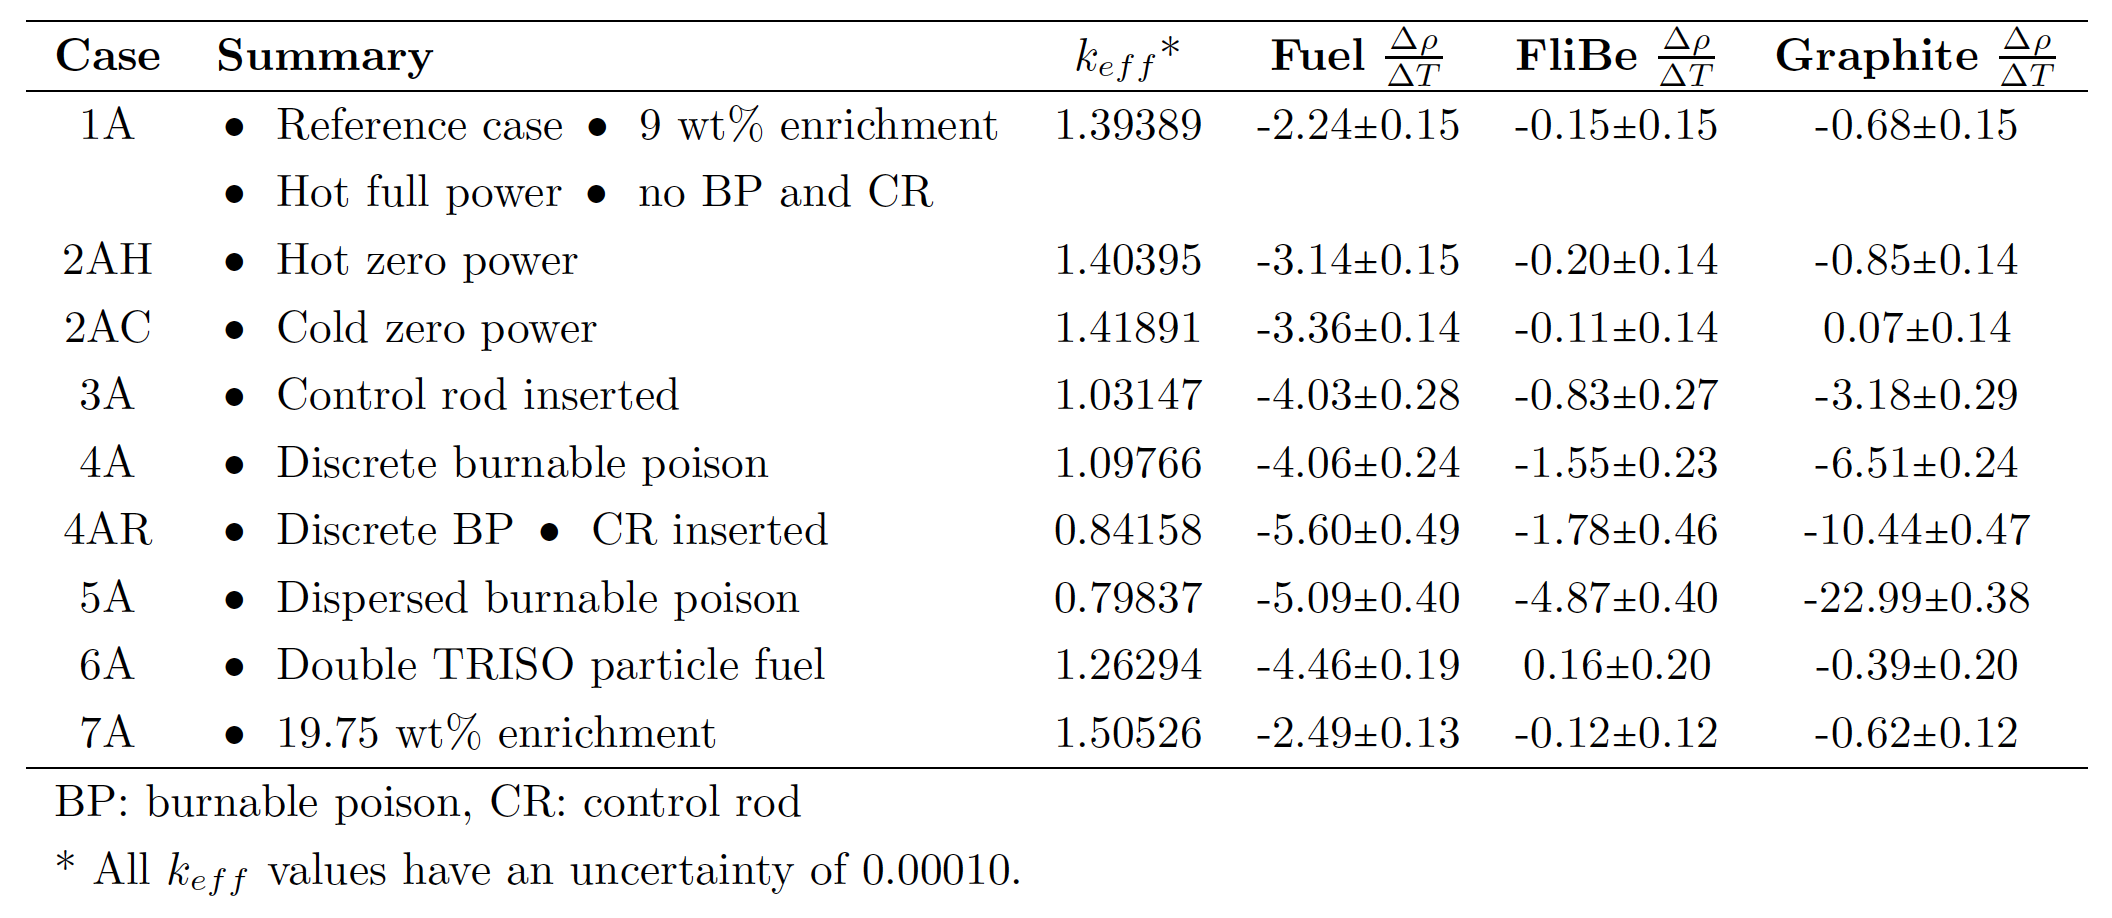
\includegraphics[width=\linewidth]{figures/benchmark-coeff-results.png}}
        \only<2>{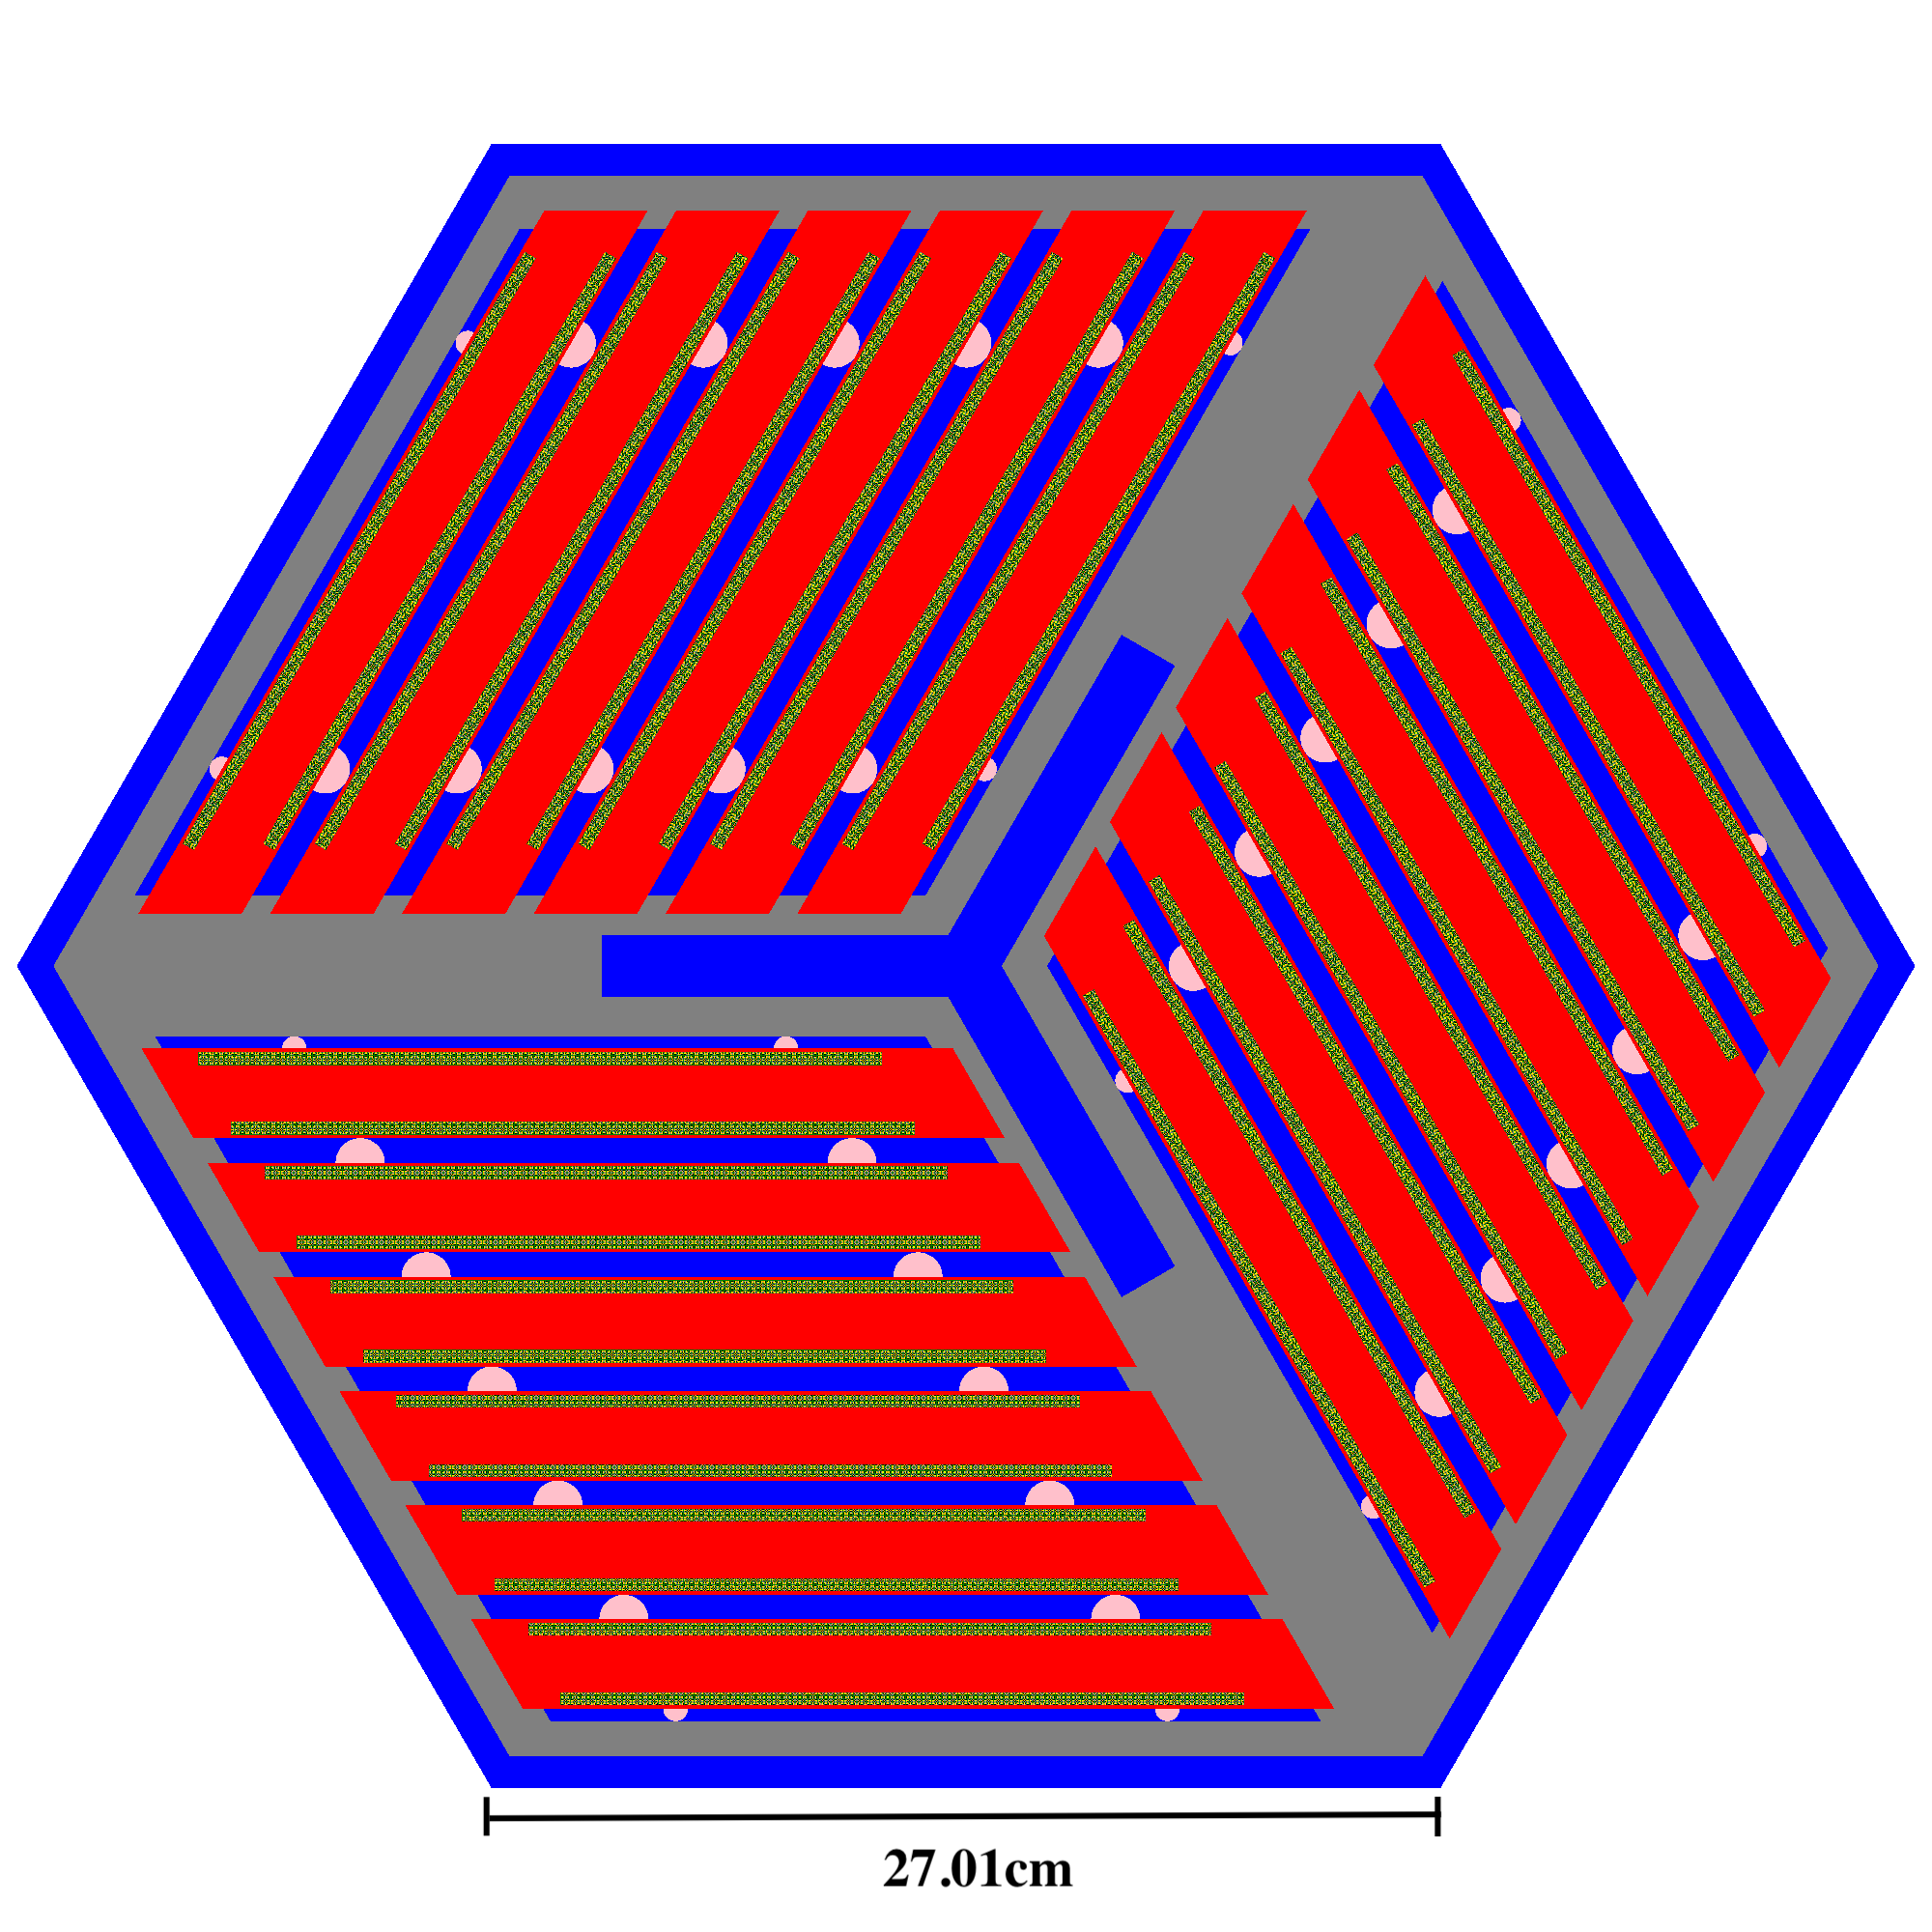
\includegraphics[width=0.6\linewidth]{../docs/figures/ahtr-fuel-element.png}}
        \only<3>{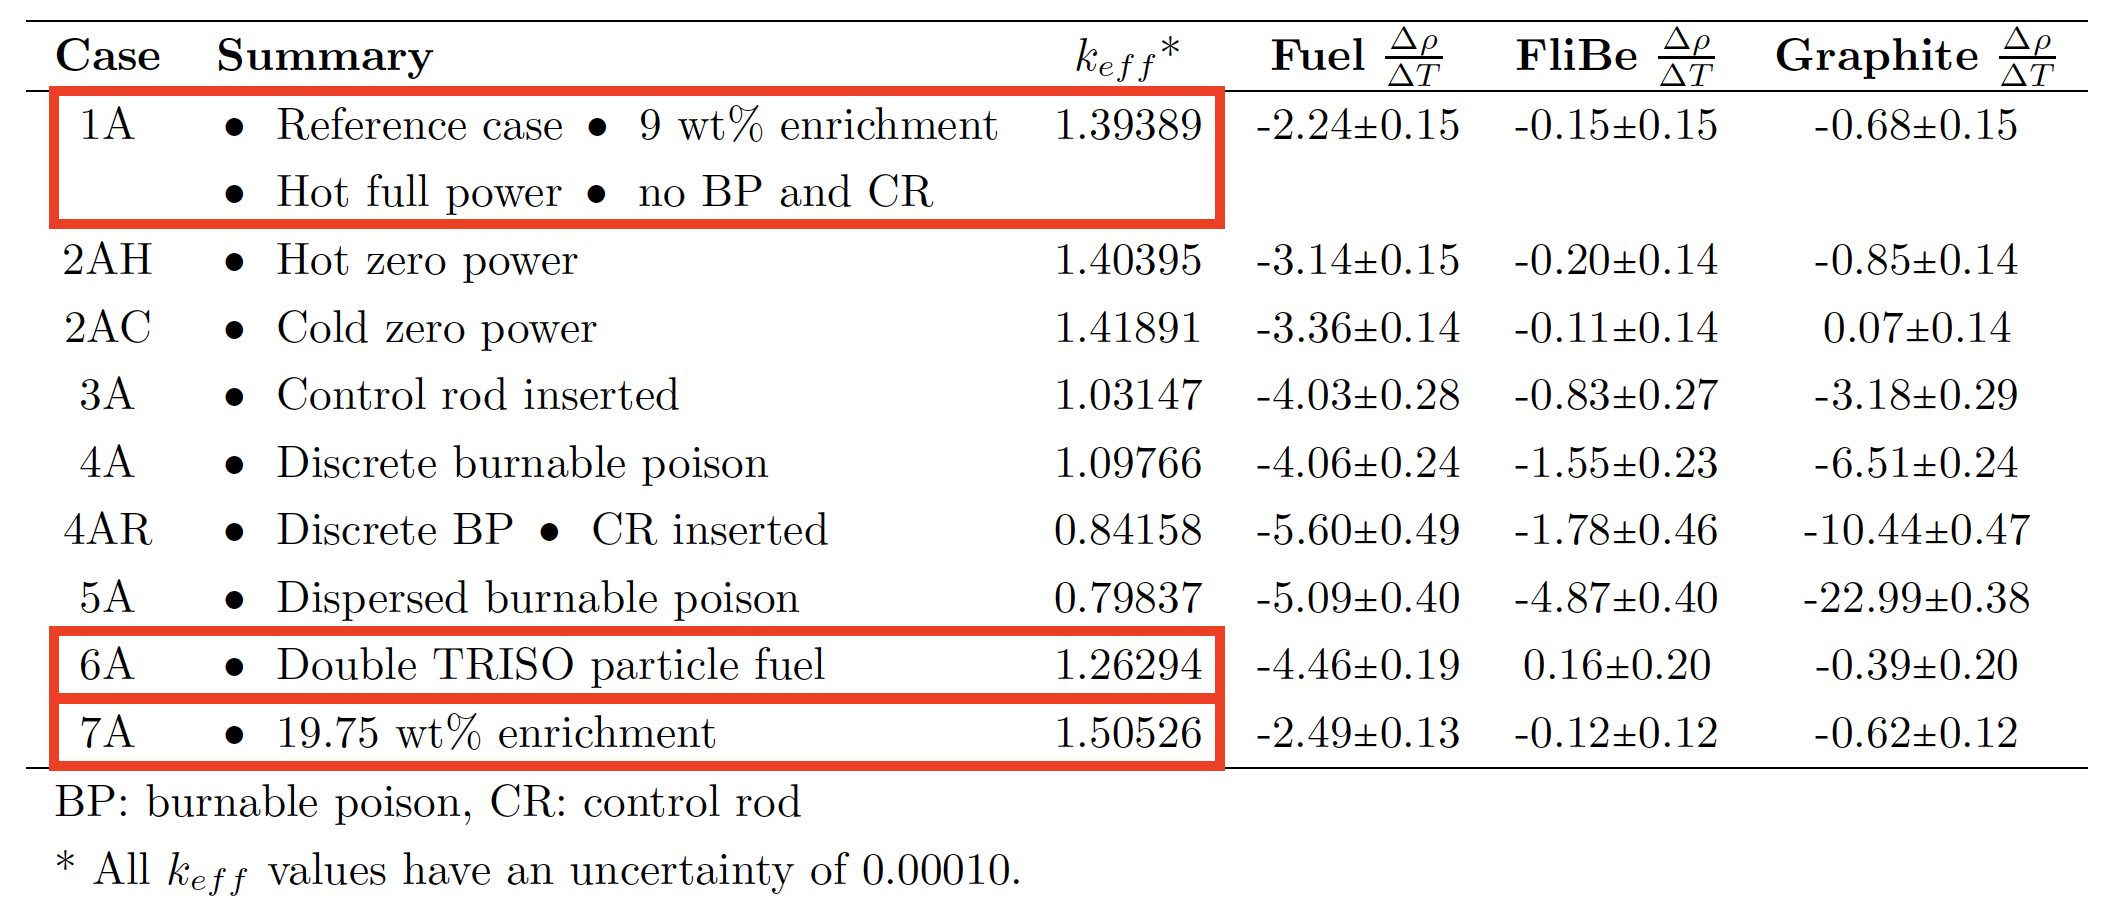
\includegraphics[width=\linewidth]{figures/benchmark-coeff-results-annotated.png}} 
        \only<4>{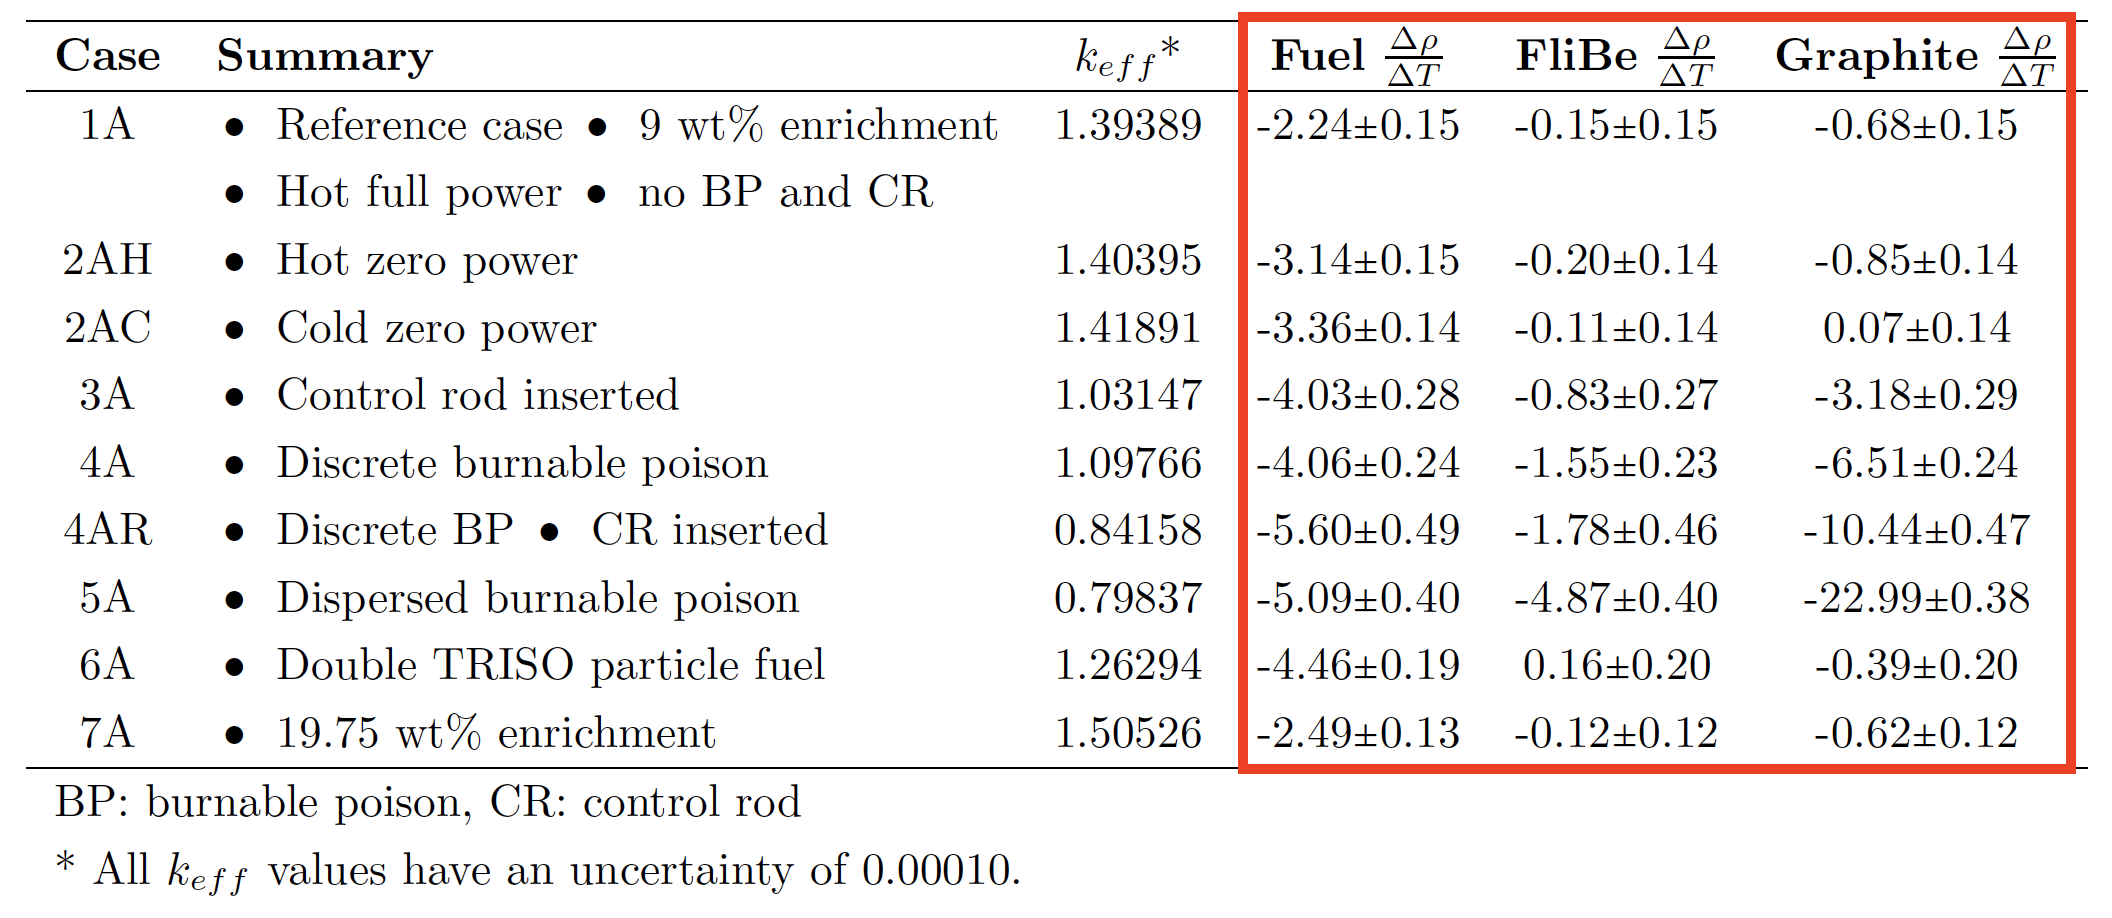
\includegraphics[width=\linewidth]{figures/benchmark-coeff-results-annotated2.png}} 
    \end{table}
    \vspace{-0.3cm}
    \only<1>{500 active cycles, 100 inactive cycles, and 200000 neutrons
    UIUC's BlueWaters supercomputer with 64 XE nodes}
    \only<3>{\textbf{Increased fuel packing does not always correspond with increased keff 
    due to spatial self-shielding effects.}}
    \only<4>{\textbf{Most of the temperature coefficients are negative, exemplifying the 
            AHTR's passive safety behavior.}}
\end{frame}

\begin{frame}
    \frametitle{FHR Benchmark Phase I-A Results}
    \vspace{-0.4cm}
    \begin{columns}
        \begin{column}{0.5\textwidth}
            \begin{figure}
                \centering
                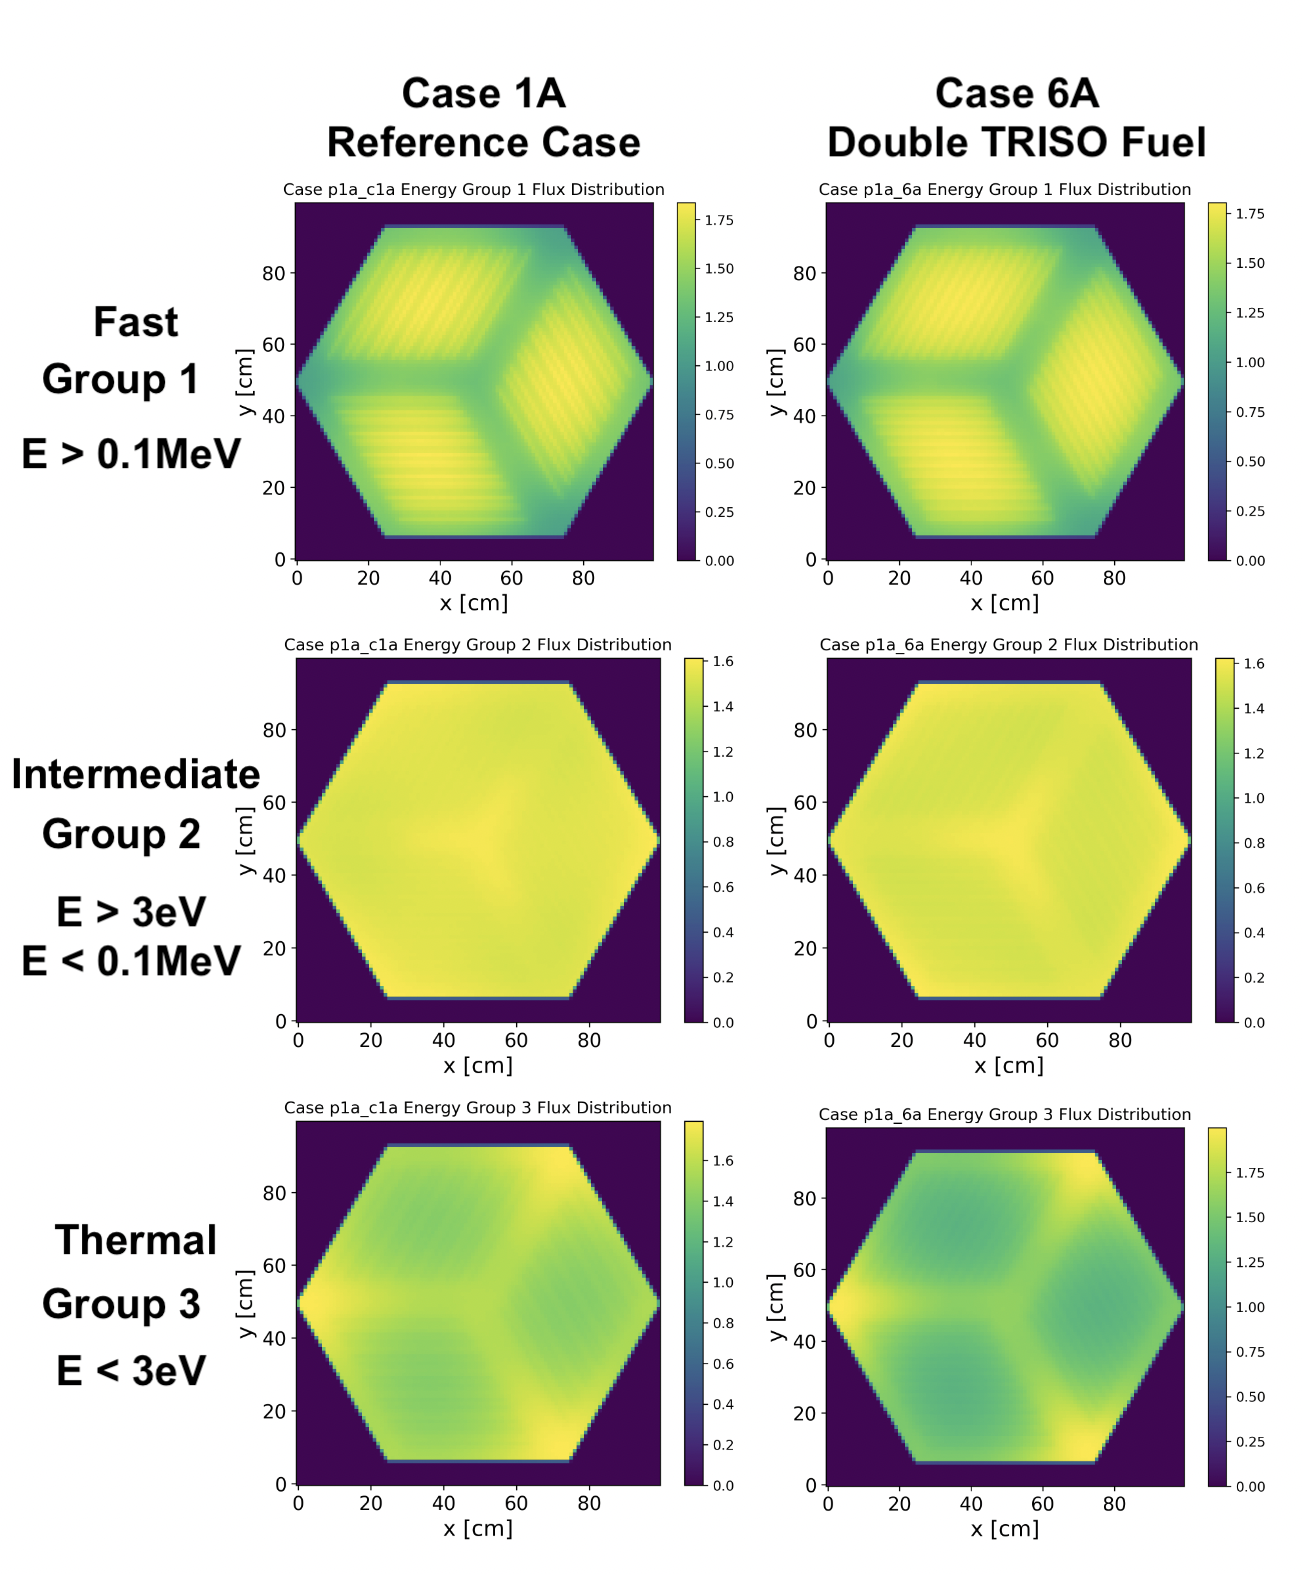
\includegraphics[width=\linewidth]{figures/phase1a-flux-vert.png} 
                \caption{Neutron flux distribution.}
            \end{figure}
        \end{column}
        \begin{column}{0.5\textwidth}
            \textbf{Key Takeaways} 
            \begin{itemize}
                \item Peak in Group 1 fast neutrons born in assembly center. Fast 
                neutrons are moderated in graphite matrix and structure 
                \item Self-shielding neutrons are more likely absorbed at the fuel 
                regions at the assembly's sides
                \item Outer sides absorb these neutrons and \textbf{geometrically 
                shield the assembly's center from neutron flux}, resulting in dip in 
                thermal Group 3 flux in the assembly's center
                \item This \textbf{self-shielding effect is more pronounced in Case 6A} 
            \end{itemize}
        \end{column}
    \end{columns}
\end{frame}

\begin{frame}
    \frametitle{FHR Benchmark Phase I-A Results}
    In an ANS M$\&$C 2021 conference paper we compared FHR benchmark participants' 
    Phase I-A results. 
    \begin{figure}[]
        \centering
        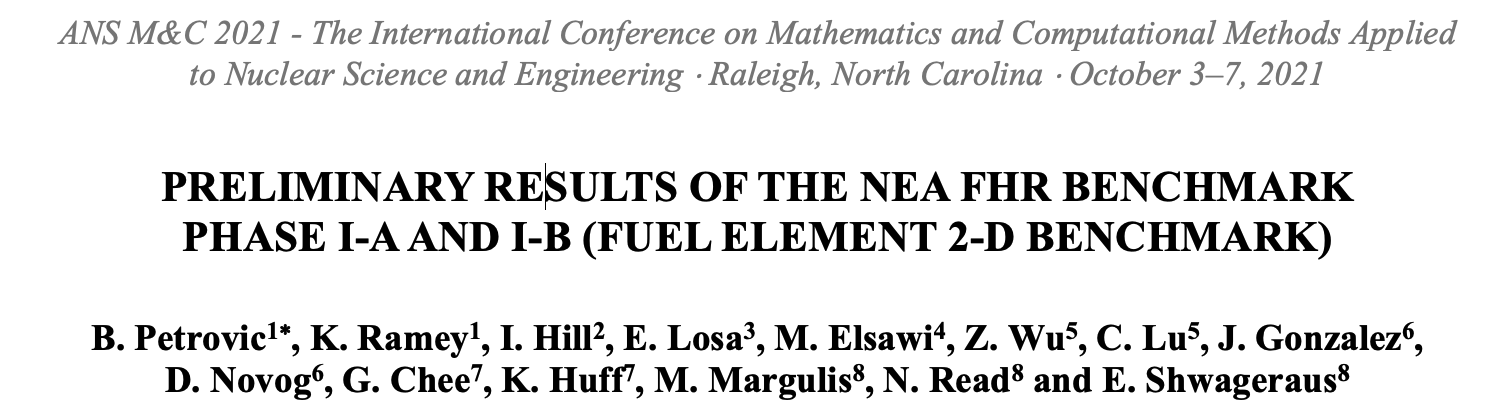
\includegraphics[width=0.85\linewidth]{figures/mnc.png} 
        \caption{FHR benchmark paper presented at M$\&$C 2021 
        \cite{petrovic_preliminary_2021}.}
    \end{figure}

    The $k_{eff}$ standard deviation between participants for each case was in the 
    231 to 514 pcm range, \textbf{acceptable and notably close} given a blind benchmark.

    \vspace{0.2cm}
    This gives \textbf{confidence to the AHTR base model's accuracy}, as I 
    proceed to optimize the AHTR for non-conventional geometries. 
\end{frame}
